\documentclass{acm_proc_article-sp}
\usepackage[utf8]{inputenc}
\usepackage{graphicx}
\newenvironment{Figure}
  {\par\medskip\noindent\minipage{\linewidth}}
  {\endminipage\par\medskip}

\begin{document}
\graphicspath{{figures/}}

\title{“Starter kit for smart buildings”}
\subtitle{Pervasive Computing : Selected Topics Project}

\numberofauthors{2} %  in this sample file, there are a *total*
% of EIGHT authors. SIX appear on the 'first-page' (for formatting
% reasons) and the remaining two appear in the \additionalauthors section.
%
\author{
\alignauthor 
  Aebischer Nadia
  \affaddr{Department of Informatics}\\
  \affaddr{University of Fribourg}\\
  \affaddr{1700 Fribourg, Switzerland}\\
  \email{nadia.aebischer@unifr.ch}
\alignauthor 
  Luyet Gil
  \affaddr{Department of Informatics}\\
  \affaddr{University of Fribourg}\\
  \affaddr{1700 Fribourg, Switzerland}\\
  \email{gil.luyet@unifr.ch}
}
\date{\today}
% Just remember to make sure that the TOTAL number of authors
% is the number that will appear on the first page PLUS the
% number that will appear in the \additionalauthors section.

\maketitle
\begin{abstract}
The goal of this report is to describe an easy way to integrate a basic pervasive system into an already built house/building. 
The system should be cheap and easy enough to integrate and to operate so it could be used by the masses as a starter kit for smart buildings. 
The report will be based on the data analysis and the context of use of this system. 
Especially about the central unit managing the whole house.
\end{abstract}


\section{Introduction}
\subsection{Smart building description}
A smart building is by definition a building enhanced by the technology that is managing it. 
Generally the technology used is splitted into four parts. 
First, we have the sensors that collect data and allow to have an understanding on what is going on outside or within the house. 
The second part is the network that allows to spread the data collected by the sensors and to eventually activate the effectors if needed. 
The third part is the managing unit that allows to gather data and infer knowledge about the environment and thus either show the data to the user or activate effectors to change the user’s environment. 
The last part is the data visualisation that allows the user to interact with the data.
This structure follows the given standard loop of a pervasive system shown in Figure \ref{loop}.
%++++++++++++++++++++++++++++++++++++++++++++++++++++++++++++++++++++++++++++
				\begin{figure}[htb]
  				\begin{center}
    				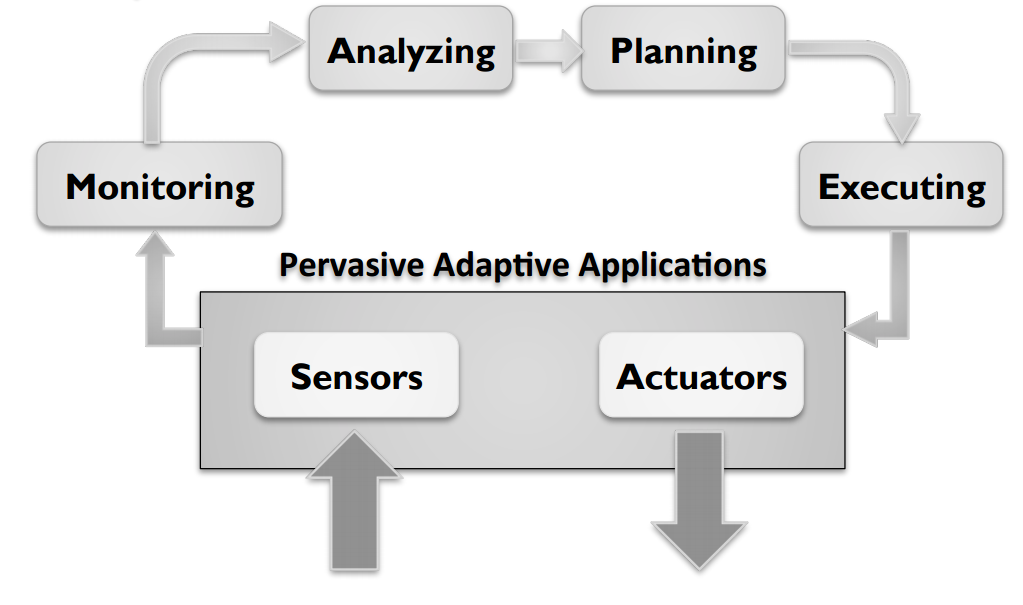
\includegraphics[width=\linewidth]{loop}
    				\caption{Pervasive system loop \label{loop}}
  				\end{center}
				\end{figure}
%++++++++++++++++++++++++++++++++++++++++++++++++++++++++++++++++++++++++++++


\subsection{Aim of the project}
The basic aim of the project is simple.
We would like to produce a simple to use and to integrate system that would allow to enhance an already built building to a smart building. 
This system should be relatively cheap and should involve the least possible physical changes in the house (e.g. destroying walls).
This means that it has to be based on cheap and already existing means and be a sort of “do-it-yourself” kit.

\section{House description}
\subsection{Context of use}
We are going to consider a small building with a dozen of individual apartments. 
Each apartment would have four rooms, each one having one light and one window with an electric sunblind. 
In such a configuration it is usual to split the power supply into so call groups. 
Each group has its own electrical phase. 
For a standard four rooms apartment (one kitchen, three rooms and one bathroom) we would have three or four groups: one managing the kitchen, one managing the bathroom and one or two groups for the other rooms. 
The building has a central water heater, separated electric meters per apartment and an individual thermostat per apartment. 
A central electrical panel is available for the whole building. An indoor parking space in common with an electric door that is activated by a remote controller is also considered.

\subsection{What could be automated}
Sunblinds are opening or closing automatically by checking the sunlight and time. 
For example if it's sunny the sunblinds will be closing. The same way, at night, they should be closing to protect our privacy.
The temperature of the apartment can also be automated. For example we can set the temperature we want to have in the apartment, 
and if the actual temperature is below or above the default one we set, the system will change the thermostat accordingly. 
We can also imagine a way to infer if somebody is going to be there soon or not and raise more or less fast the overall temperature. 
This inference can be computed according to the presence of people in the house by reading the presence sensors. 
For example, if somebody is never present during the weekends then the central unit should over the time learn that fact and thus it will heat the apartment in order to saving energy.
The lights can also be automated by detecting the presence of people in a room.
RFID tags linked with cars could be used to open the parking space doors.
Of course, these automated behaviors can be stopped by the user if he doesn't want it to be performed. 
To do so, the user can access the central unit via a web interface and change the behavior the way he want at all times.

	
\section{A few words about the sensors}
In this section, we will briefly talk about the different sensors that our Central Unit will deal with. 
We are not going into too much details as it is not our main subject for this project.
\subsection{Sensors architecture}
The communication between the components are achieved by WiFi or over the electrical network in case the WiFi is not reachable. 
Communication over the electrical network can achieve a very fast connection speed between the components, up to 1200 Mbits/s [1]. % TODO: add reference from Devolo website!
This means that theoretically preprocessing of sensors data is not needed but for utility reasons we will preprocess the data before reaching the Central Unit.
Each sensor is connected to a light computer, typically a Raspberry Pi could work but we can imagine an even less powerful one for small tasks. 
This light computer will preprocess the raw sensor data and play the role of the interface between the sensor and the Central Unit. 
This interface is needed in case of multiple types of sensors. By changing the sensors, one could simply apply a patch to the small computer (even via the Central Unit) and resolve compatibility issues. 
This interface used here is a simple HTTP based communication via POST with a specific XML-based body very similar to the SOAP protocol:
\begin{verbatim}
POST address 
  <MESSAGE>
    <TYPE>(alert|event|failure|do)</TYPE>
    <FROM>(sensor_id|central)</FROM>
    <CONTENT/>
  </MESSAGE>
\end{verbatim}
Where the \texttt{TYPE} denotes an alert, an event or even a failure for example. 
The \texttt{FROM} and \texttt{CONTENT} parts deals respectively with the author of the message and the actual meaning of the message. 
A typical proximity sensor message would look like the following:
\begin{verbatim}
POST address_of_CentralUnit 
  <MESSAGE>
    <TYPE>event</TYPE>
    <FROM>sensor_id2345</FROM>
    <CONTENT>distance:'2.34m'</CONTENT/>
  </MESSAGE>
\end{verbatim}
A typical message sent by the Central Unit to open a door would be:
\begin{verbatim}
POST address_of_door_effector
  <MESSAGE>
    <TYPE>do</TYPE>
    <FROM>central</FROM>
    <CONTENT>door[0]:'open'</CONTENT/>
  </MESSAGE> 
\end{verbatim}


\subsection{Location}
The locations of the sensors depend of the type of sensor. Here is the list of the sensors we are going to consider:
\begin{description}
 \item[Luminosity sensor] - outside, at each frontage of the house.
 \item[Presence sensors] - around the lights and the doors.
 \item[Temperature sensors] - inside/outside.
 \item[Energy consumption sensor] - after the electric meter.
 \item[Water consumption sensor] - before the water inlet.
 \item[Water temperature sensor] - after the water heater.
 \item[RFID readers] - for cars around the garage doors.
\end{description}
We also consider effectors, the list of them is given here:
\begin{description}
 \item[Sunblinds effectors] - to open and close sunblinds.
 \item[Light effectors] - to switch the lights on and off.
 \item[Thermostat effector] - to change the house temperature.
 \item[Automatic garage door opener] - to be linked with the RFID reader.
\end{description}
This part is not really important for the scope we choose to aim our report, but this should be at least mentioned because it lists which sensors we are going to consider and we are receiving data from in order to form a context, and also on which effectors the Central Unit can send message to change the environment.
\section{Central Unit}	
The Central Unit is the main part of this architecture and the scope of this report. 
This Central Unit depends on several topics as its own architecture, the sensors data coming in, 
the effectors it has to interact with its environment and of course its standard interface with the user.
\subsection{Architecture of central unit}
The architecture itself has no specific requirement. 
We can choose whatever we want, here we might focus on a standard Linux distribution as Ubuntu without any graphical environment as the only interaction we have will be via a web interface discussed later. 
Furthermore the computation needed is not too high as the preprocessing of the sensor is done on the sensor side with light computer as discussed earlier. 
The computer should also be running 24/7 and thus the computer has to have a low consumption. A light computer as a Raspberry Pi might be enough.


\subsection{Sensor fusion}
The sensors fusion is performed to produce a context. A context is the actual state of an entity such as a room or a person. In this report we need to know exactly which kind of contexts we are going to consider to know exactly which sensor data has to be aggregated to produce the actual state of a room for example. Here are the contexts we are going to consider:
\begin{description}
 \item[The lightning state of the room]\hfill \\ 
 Is the room dark or enlighted ? Does the lights are activated ? This information can
 be infered by using the inside and outside lightning sensors, sunblinds status and the lights status.
 \item[The occupation of the room]\hfill \\ 
 Is the room empty or not. When does the room is usually empty ?
 \item[The actual weather state inside and outside]\hfill \\
 (temperature, lightning and precipitations). 
 Is the temperature cold/warm, based on a threshold. Is the temperature cooler or warmer outside ? 
 Does it rain/snow outside ? What is the actual lightning ?
 \item[Which is the part of the day ?] \hfill \\
 Look at the actual time => infers moning / evening / midnight / ...
 \item[Is a car waiting at the garage doors ?] \hfill \\
  Look at the RFID reader. Is the car allowed to pass ?
 \item[What is the actual consumption of the whole building ?]\hfill \\
 May be used to display to the webinterface.
\end{description}
\textbf{[INSERT HERE WHY THOSE CONTEXTS]}\\
As this list is now fully established we have to on which sensors to use to analyse the context wanted.
\begin{itemize}
 \item The lightning state of the room: .
 \item The occupation of the room: Presence sensors.
 \item The actual weather state: Regional meteo status available over the internet.
 \item Is a car waiting at the parking doors: RFID reader near the garage doors.
 \item What is the actual consumption of the whole building: Energy consumption sensor and water consumption sensor
\end{itemize}
Admit now that each context has been computer via the sensor data. We must now describe how an actual context combined with new sensors data coming in will react. This can be done via listening all the possibilities.
\begin{description}
 \item[Do] activate lightning \textbf{if} somebody enters the room $\land$ the room is dark.
 \item[Do] deactivate lightning \textbf{if} the room becomes empty $\land$ the room is lightened.
 \item[Do] reduce heating \textbf{if} room is usually empty for a quite long period $\land$ nobody is inside.
 \item[Do] reduce heating \textbf{if} outside temperature > comfort temperature $\pm$ threshold
 \item[Do] augment heating \textbf{if} temperature < comfort temperature $\pm$ threshold.
 \item[Do] open doors \textbf{if} car is at the parking doors $\land$ door closed.
 \item[Do] close the doors \textbf{if} timer for doors is over $\land$ no car at the parking doors.
 \item[Do] close sunblinds \textbf{if} lightning outside < threshold $\land$ part of the day!=’day’.
 \item[Do] open sunblinds \textbf{if} sunblinds closed $\land$ part of the day=’day’ $\land$ someone enters the room.
\end{description}

\subsection{Effectors}
Automation of control. Inference for temperature calculation by knowing is somebody usually will come to the house.
\subsection{Web-based manual controller}
for mobile + desktop + over Internet
stats presentations
failure presentations
notifications (SMS, e-mail, Facebook, invasive smartphone application)
	what must be stopped
	what must be switched on/off automatically
	crash of computer (?) : keep some switches ?




\section{Conclusion}




\section{Acknowledgments}



%\nocite{*}
% The following two commands are all you need in the
% initial runs of your .tex file to
% produce the bibliography for the citations in your paper.
%\bibliographystyle{abbrv}
%\bibliography{sigproc}  % sigproc.bib is the name of the Bibliography in this case

\end{document}
